\ifx\allfiles\undefined
\documentclass[12pt, a4paper,oneside, UTF8]{ctexbook}
\usepackage[dvipsnames]{xcolor}
\usepackage{mathtools}   % 数学公式(mathtools 是 amsmath 的上位替代)
\usepackage{amsthm}    % 定理环境
\usepackage{amssymb}   % 更多公式符号
\usepackage{graphicx}  % 插图
%\usepackage{mathrsfs}  % 数学字体
%\usepackage{newtxtext,newtxmath}
%\usepackage{arev}
\usepackage{kmath,kerkis}
\usepackage{newtxtext}
\usepackage{bbm}
\usepackage{enumitem}  % 列表
\usepackage{geometry}  % 页面调整
%\usepackage{unicode-math}
\usepackage[colorlinks,linkcolor=black]{hyperref}

\usepackage{wrapfig}


\usepackage{ulem}	   % 用于更多的下划线格式,
					   % \uline{}下划线,\uuline{}双下划线,\uwave{}下划波浪线,\sout{}中间删除线,\xout{}斜删除线
					   % \dashuline{}下划虚线,\dotuline{}文字底部加点


\graphicspath{ {flg/},{../flg/}, {config/}, {../config/} }  % 配置图形文件检索目录
\linespread{1.5} % 行高

% 页码设置
\geometry{top=25.4mm,bottom=25.4mm,left=20mm,right=20mm,headheight=2.17cm,headsep=4mm,footskip=12mm}

% 设置列表环境的上下间距
\setenumerate[1]{itemsep=5pt,partopsep=0pt,parsep=\parskip,topsep=5pt}
\setitemize[1]{itemsep=5pt,partopsep=0pt,parsep=\parskip,topsep=5pt}
\setdescription{itemsep=5pt,partopsep=0pt,parsep=\parskip,topsep=5pt}

% 定理环境
% ########## 定理环境 start ####################################
\theoremstyle{definition}
\newtheorem{defn}{\indent 定义}[section]

\newtheorem{lemma}{\indent 引理}[section]    % 引理 定理 推论 准则 共用一个编号计数
\newtheorem{thm}[lemma]{\indent 定理}
\newtheorem{corollary}[lemma]{\indent 推论}
\newtheorem{criterion}[lemma]{\indent 准则}

\newtheorem{proposition}{\indent 命题}[section]
\newtheorem{example}{\indent \color{SeaGreen}{例}}[section] % 绿色文字的 例 ,不需要就去除\color{SeaGreen}{}
\newtheorem*{rmk}{\indent \color{red}{注}}

% 两种方式定义中文的 证明 和 解 的环境:
% 缺点:\qedhere 命令将会失效【技术有限,暂时无法解决】
\renewenvironment{proof}{\par\textbf{证明.}\;}{\qed\par}
\newenvironment{solution}{\par{\textbf{解.}}\;}{\qed\par}

% 缺点:\bf 是过时命令,可以用 textb f等替代,但编译会有关于字体的警告,不过不影响使用【技术有限,暂时无法解决】
%\renewcommand{\proofname}{\indent\bf 证明}
%\newenvironment{solution}{\begin{proof}[\indent\bf 解]}{\end{proof}}
% ######### 定理环境 end  #####################################

% ↓↓↓↓↓↓↓↓↓↓↓↓↓↓↓↓↓ 以下是自定义的命令  ↓↓↓↓↓↓↓↓↓↓↓↓↓↓↓↓

% 用于调整表格的高度  使用 \hline\xrowht{25pt}
\newcommand{\xrowht}[2][0]{\addstackgap[.5\dimexpr#2\relax]{\vphantom{#1}}}

% 表格环境内长内容换行
\newcommand{\tabincell}[2]{\begin{tabular}{@{}#1@{}}#2\end{tabular}}

% 使用\linespread{1.5} 之后 cases 环境的行高也会改变,重新定义一个 ca 环境可以自动控制 cases 环境行高
\newenvironment{ca}[1][1]{\linespread{#1} \selectfont \begin{cases}}{\end{cases}}
% 和上面一样
\newenvironment{vx}[1][1]{\linespread{#1} \selectfont \begin{vmatrix}}{\end{vmatrix}}

\def\d{\textup{d}} % 直立体 d 用于微分符号 dx
\def\R{\mathbb{R}} % 实数域
\def\N{\mathbb{N}} % 自然数域
\def\C{\mathbb{C}} % 复数域
\def\Z{\mathbb{Z}} % 整数环
\def\Q{\mathbb{Q}} % 有理数域
\newcommand{\bs}[1]{\boldsymbol{#1}}    % 加粗,常用于向量
\newcommand{\ora}[1]{\overrightarrow{#1}} % 向量

% 数学 平行 符号
\newcommand{\pll}{\kern 0.56em/\kern -0.8em /\kern 0.56em}

% 用于空行\myspace{1} 表示空一行 填 2 表示空两行  
\newcommand{\myspace}[1]{\par\vspace{#1\baselineskip}}

%s.t. 用\st就能打出s.t.
\DeclareMathOperator{\st}{s.t.}

%罗马数字 \rmnum{}是小写罗马数字, \Rmnum{}是大写罗马数字
\makeatletter
\newcommand{\rmnum}[1]{\romannumeral #1}
\newcommand{\Rmnum}[1]{\expandafter@slowromancap\romannumeral #1@}
\makeatother
\begin{document}
	% \title{{\Huge{\textbf{$Partial \,\, Differential \,\, Equations$}}}\footnote{参考书籍:\\
			\hspace*{4em} \textbf{《Partial Differential Equations》 -- Lawrence C. Evans} \\
			\hspace*{4em} \textbf{《Partial Differential Equations》 -- Fritz John} \\
			\hspace*{4em} \textbf{《数学物理方程讲义 (第二版)》--  姜礼尚、陈亚浙、刘西垣、易法槐} 
			}}
\author{$-TW-$}
\date{\today}
\maketitle                   % 在单独的标题页上生成一个标题

\thispagestyle{empty}        % 前言页面不使用页码
\begin{center}
	\Huge\textbf{序}
\end{center}


\vspace*{3em}
\begin{center}
	\large{\textbf{天道几何,万品流形先自守;}}\\
	
	\large{\textbf{变分无限,孤心测度有同伦。}}
\end{center}

\vspace*{3em}
\begin{flushright}
	\begin{tabular}{c}
		\today \\ \small{\textbf{长夜伴浪破晓梦,梦晓破浪伴夜长}}
	\end{tabular}
\end{flushright}


\newpage                      % 新的一页
\pagestyle{plain}             % 设置页眉和页脚的排版方式(plain:页眉是空的,页脚只包含一个居中的页码)
\setcounter{page}{1}          % 重新定义页码从第一页开始
\pagenumbering{Roman}         % 使用大写的罗马数字作为页码
\tableofcontents              % 生成目录

\newpage                      % 以下是正文
\pagestyle{plain}
\setcounter{page}{1}          % 使用阿拉伯数字作为页码
\pagenumbering{arabic}
\setcounter{chapter}{0}    % 设置 -1 可作为第零章绪论从第零章开始 
	\else
	\fi
	%  ############################ 正文部分
\appendix
\chapter{$Supplementary \,\, Content$}\label{appendix A}

\section{区域边界的光滑性}
	下面我们来给出\textbf{区域边界的光滑性}的定义.
	
	\begin{defn}\label{def A.1.1}
		Suppose $\Omega \subset \R^n$ is open, $\partial \Omega \neq \varnothing$. 如果对于$\forall p \in \partial \Omega$, $\exists p$ 的邻域$U$, $\st$ 在适当的空间直角坐标系下, 
		\begin{align}
			\partial \Omega \cap U &= \{ (x^{'} , x^{n}) \in \R^{n - 1} \times \R \mid x^{'} \in D , \,\, x^n = \varphi(x^{'}) \} \\
			\Omega \cap U &= \{ (x^{'} , x^n) \in \R^{n - 1} \times \R \mid x^{'} \in D , \,\, x^n > \varphi(x^{'}) \} \cap U
		\end{align}
		where $\varphi \in C^{k}(\Omega) , \,\, D \subset \R^{n - 1}$ open. 我们称\underline{\textcolor{blue}{\textbf{$\partial \Omega \in C^k$}}}, 这里$k = 0 , 1 , 2 , \cdots$ 或$\infty$.
		
		\begin{figure}[thbp!]
			\centering
			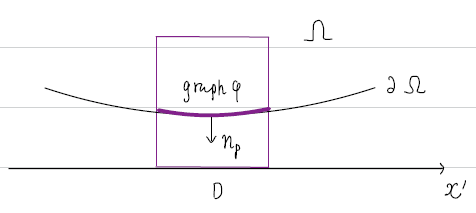
\includegraphics[width=0.5\linewidth]{figure/A.1-1}
			\caption{边界的光滑性}
			\label{pic : A.1-1} % 添加图像引用标签
		\end{figure}
		
		\begin{rmk}
			在\textbf{定义 \ref{def A.1.1}} 中, 设$k \leq 1$, $\,\, x_{0}^{'} \in \partial \Omega$, $\,\, p = (x_{0}^{'} , \varphi(x_{0}^{'}))$. 记
			\[ n_p = \frac{(\nabla \varphi(x_{0}^{'}) , -1)}{\sqrt{1 + \left| \nabla \varphi(x_{0}^{'}) \right|^2}} \]
			称$n_p$ 为$\partial \Omega$ 在$p$ 点的\underline{\textcolor{blue}{\textbf{单位外法向}}}. $n_p$ 的定义与空间直角坐标系的选择无关. 记
			\begin{align}
				n : \partial \Omega &\longrightarrow \R^n \\
				p &\longmapsto n(p) = n_p 
			\end{align}
			称$n$ 为$\partial \Omega$ 的\underline{\textcolor{blue}{\textbf{单位外法向}}}. 因为$\partial \Omega \in C^k$, $k \geq 1$, 所以$n \in C(\partial \Omega ; \R^n)$.
		\end{rmk}
	\end{defn}

\newpage

\section{含参变量的积分}
	在分析中, 我们常遇到如下形式的积分定义的函数:
	\[ \varphi(x) = \int_{c}^d f(x , t) \, dt , \,\, x \in [a , b] \]
	上式右端的积分称为\textbf{含参变量 (参变量为$x$) 的积分}. 下面我们来给出由含参变量的积分所定义的函数的\textbf{连续性}、\textbf{可积性}和\textbf{可微性}. 
	
	\begin{thm}\label{thm A.2.1}
		设$f \in C([a , b] \times [c , d])$. 记$\varphi : [a , b] \longrightarrow \R$, 
		\[ \varphi(x) = \int_{c}^d f(x , t) \, dt , \,\, \forall x \in [a , b] \]
		则
		\begin{enumerate}
			\item[(\rmnum{1})] $\varphi \in C[a , b]$. 
			
			\item[(\rmnum{2})] If $D_{1}f \in C([a , b] \times [c , d])$, then $\varphi \in C^{1}([a , b])$ and 
			\[ \varphi^{'}(x) = \int_{c}^d D_{1}f(x , t) \,  dt , \,\, \forall x \in [a , b] \]
			
			\item[(\rmnum{3})] $\varphi$ Riemann可积, 并且
			\[ \int_{a}^b \varphi = \int_{c}^d \left( \int_{a}^b f(x , t) \, dx \right) \, dt \]
		\end{enumerate}
	
		\vspace{4em}
		
		\begin{rmk}
			\begin{itemize}
				\item (\rmnum{1})中$\varphi \in C[a , b]$ 表明了\textbf{积分与极限可交换次序}, 即
				\[ \lim_{x \to x_0} \int_{c}^d f(x , t) \, dt = \int_{c}^d \lim_{x \to x_0} f(x , t) \, dt = \int_{c}^d f(x_0 , t) \, dt , \,\, \forall x_0 \in [a , b] \]
				同理, (\rmnum{2})和(\rmnum{3})也分别告诉我们\textbf{求导和积分、积分和积分之间可交换次序}.
				
				\vspace{4em}
				
				\item 根据数学归纳法, 如果$f \in C^{k}([a , b] \times [c , d])$, 则$\varphi \in C^{k}[a , b]$, 
				\[ \varphi^{(i)}(x) = \int_{c}^d \frac{d^i}{d x^i} f(x , t) \, dt , \,\, \forall i = 1 \sim k \]
				即\textbf{任意$k$ 阶内积分与求导可交换次序}, 即
				\[ \frac{d^i}{dx^{i}} \int_{c}^d f(x , t) \, dt = \int_{c}^d \frac{d^i}{d x^i} f(x , t) \, dt , \,\, \forall i = 1 \sim k \]
			\end{itemize}
		\end{rmk}
	\end{thm}

\newpage

\section{含参变量的广义积分的一致收敛}
	为了考察\textbf{含参变量的广义积分的连续性、可积性和可微性}, 我们先来给出\textbf{含参变量广义积分的一致收敛}的概念.
	
	\begin{defn}\label{def A.3.1}
		设$f : D \times [a , \infty) \longrightarrow \R$, 对于$\forall x \in D$, $b > a$, $f(x , \cdot)$ 在$[a , b]$ 上Riemann可积. 如果对于$\forall x \in D$, 积分$\int_{a}^{\infty} f(x , t) \, dt$ 收敛, 并且对于$\forall \epsilon > 0$, $\exists M > a$, $\st$
		\[ \left| \int_{A}^{\infty} f(x , t) \, dt \right| \leq \epsilon , \,\, \forall A > M , \,\, \forall x \in D \]
		称\underline{\textcolor{blue}{\textbf{积分$\int_{a}^\infty f(x , t) \, dt$ 关于$x$  一致收敛}}}. 
		
		\vspace{4em}
		
		\begin{rmk}
			\begin{itemize}
				\item 设$A > a$. Let
				\begin{align}
					\varphi(x) &= \int_{a}^{\infty} f(x , t) \, dt , \,\, x \in D \\
					\widetilde{\varphi}(x) &= \int_{a}^A f(x , t) \, dt , \,\, x \in D
				\end{align}
				由定义, 如果积分$\int_{a}^\infty f(x , t) \, dt$ 关于$x$ 一致收敛, 则当$A$ 充分大时, 积分$\int_{a}^{\infty} f(x , t) \, dt$ 关于$x$ 一致地小. 此时
				\[ \varphi(x) = \int_{a}^A f(x , t) \, dt + \int_{A}^{\infty} f(x , t) \, dt \approx \widetilde{\varphi}(x) \]
				所以我们可以期望
				\begin{center}
					\textbf{一致收敛的}由含参变量的无穷限积分所定义的函数$\varphi$ \\
					与 \\
					由含参变量的常义积分所定义的$\widetilde{\varphi}$ 有相同的性质.
				\end{center}
				
				\vspace{4em}
				
				\item $\forall a_1 > a$, 
				\begin{center}
					$\int_{a}^{\infty} f(x , t) \, dt$ 一致收敛 $\,\, \Leftrightarrow \,\, \int_{a_1}^{\infty} f(x , t) \, dt$ 一致收敛
				\end{center}
			\end{itemize}
		\end{rmk}
	\end{defn}

\newpage

	下面给出判定积分$\int_{a}^{\infty} f(x , t) \, dt$ 是否一致收敛的一些判定准则. 

	\begin{proposition}\label{prop A.3.1}
		\textbf{[Cauchy收敛原理]}. \\
		设$f : D \times [a , \infty) \longrightarrow \R$, 对于$\forall x \in D$, $b > a$, $f(x , \cdot)$ 在$[a , b]$ 上Riemann可积, 则
		\begin{center}
			积分$\int_{a}^\infty f(x , t) \, dt$ 一致收敛 $\,\, \Leftrightarrow \,\,$ 对于$\forall \epsilon > 0$, $\exists M > a$, $\st$
			\[ \left| \int_{A_1}^{A_2} f(x , t) \, dt \right| \leq \epsilon , \,\, \forall A_2 > A_1 \geq M , \,\, \forall x\ in D \]
		\end{center}
	\end{proposition}

	\vspace{8em}

	\begin{proposition}\label{prop A.3.2}
		\textbf{[比较判别法]}. \\
		设$f : D \times [a , \infty) \longrightarrow \R$, 对于$\forall x \in D$, $b > a$, $f(x , \cdot)$ 在$[a , b]$ 上Riemann可积. 设$g : [a , \infty) \longrightarrow \R$, $g \geq 0$, 对于$\forall b > a$, $g$ 在$[a , b]$ 上Riemann可积. 如果
		\[ \left| f(x  ,t) \right| \leq g(t) , \,\, \forall (x ,t) \in D \times [a , \infty) \]
		并且$\int_{a}^{\infty} g(t) \, dt < \infty$, 则积分$\int_{a}^{\infty} f(x , t) \, dt$ 一致收敛.
	\end{proposition}

	\vspace{8em}
	
	\begin{proposition}\label{prop A.3.3}
		\textbf{[Dirichlet判别法]}. \\
		设$f , g : D \times [a , \infty) \longrightarrow \R$, 对于$\forall x \in D$, $b > a$, $f(x , \cdot) , g(x , \cdot)$ 在$[a , b]$ 上Riemann可积. 设对于$\forall x \in D$, $g(x , \cdot)$ 单调. 如果
		\begin{enumerate}
			\item[(\rmnum{1})] $\forall \epsilon > 0$, $\exists M > a$, $\st$
			\[ \left| g(x , t) \right| \leq \epsilon , \,\, \forall t \geq M , x \in D \]
			
			\item[(\rmnum{2})] $\exists L \in \R$, $\st$
			\[ \left| \int_{a}^b f(x , t) \, dt \right| \leq L , \,\, \forall b \geq a , \,\, \forall x \in D \]
		\end{enumerate}
		则积分$\int_{a}^{\infty} f(x , t) g(x , t) \, dt$ 一致收敛.
	\end{proposition}
	
	\newpage
	
	\begin{proposition}\label{prop A.3.4}
		\textbf{[Abel判别法]}. \\
		设$f , g : D \times [a , \infty) \longrightarrow \R$, 对于$\forall x \in D$, $b > a$, $f(x , \cdot) , g(x , \cdot)$ 在$[a , b]$ 上Riemann可积. 设对于$\forall x \in D$, $g(x , \cdot)$ 单调. 如果
		\begin{enumerate}
			\item[(\rmnum{1})] $\exists L \in \R$, $\st$
			\[ \left| g(x , t) \right| \leq L , \,\, \forall (x  , t) \in D \times [a , \infty) \]
			
			\item[(\rmnum{2})] 积分$\int_{a}^\infty f(x , t) \, dt$ 一致收敛
		\end{enumerate}
		则积分$\int_{a}^{\infty} f(x , t) g(x , t) \, dt$ 一致收敛.
	\end{proposition}

\newpage

\section{含参变量的广义积分的性质}
	下面讨论由含参变量的广义积分所定义的函数的\textbf{连续性}、\textbf{可积性}和\textbf{可微性}, 即\textbf{积分与极限交换次序}、\textbf{积分与积分交换次序}、\textbf{积分与求导交换次序}的问题. 
	
	\vspace{1em}
	
	首先给出\textbf{一致收敛}时积分$\int_{c}^{\infty} f(x , t) \, dt$ 的\textbf{连续性}和\textbf{可积性}. 
	
	\begin{proposition}\label{prop A.4.1}
		设$f \in C([a , b] \times [c , \infty])$. 设积分$\int_{c}^{\infty} f(x , t) \, dt$ 关于$x$ 一致收敛. 记
		\[ \varphi(x) = \int_{c}^{\infty} f(x , t) \, dt , \,\, \forall x \in [a , b] \]
		则
		\begin{enumerate}
			\item[(\rmnum{1})] $\varphi \in C[a , b]$. 
			
			\item[(\rmnum{2})] 积分$\int_{c}^{\infty} \left( \int_{a}^b f(x , t) \, dx \right) \, dt$ 收敛, 并且
			\[ \int_{a}^b \varphi = \int_{c}^{\infty} \left( \int_{a}^b f(x , t) \, dx \right) \, dt \]
		\end{enumerate}
	\end{proposition}

	\vspace{12em}
	
	下面再给出积分$\int_{c}^{\infty} f(x , t) \, dt$ 的\textbf{可微性}.
	
	\begin{proposition}\label{prop A.4.2}
		设$f : [a , b] \times [c , d] \longrightarrow \R , \,\, f , D_{1}f \in C([a , b] \times [c  ,d])$. 如果
		\begin{center}
			\begin{enumerate}
				\item[(\rmnum{1})] $\exists x_0 \in [a , b]$, $\st$ 积分$\int_{c}^{\infty} f(x_0 , t) \, dt$ 收敛.
				
				\item[(\rmnum{2})] 积分$\int_{c}^{\infty} D_{1}f(x , t) \, dt$ 关于$x$ 一致收敛.
			\end{enumerate}
		\end{center}
		则积分$\int_{c}^{\infty} f(x , t) \, dt$ 关于$x$ 一致收敛. 记
		\[ \varphi(x) = \int_{c}^{\infty} f(x , t) \, dt , \,\, \forall x \in [a , b] \]
		则$\varphi \in C^{1}[a , b]$, 并且
		\[ \varphi^{'}(x) = \int_{c}^{\infty} D_{1}f(x , t) \, dt , \,\, \forall x \in [a , b] \]
	\end{proposition}

	\newpage
	
	根据\textbf{命题 \ref{prop A.4.2}}, 运用数学归纳法可得到如下推论.
	
	\begin{corollary}\label{cor A.4.1}
		设$f \in C^{k}([a , b] \times [c , d])$, $k \in \N$. 设积分
		\[ \int_{c}^{\infty} \frac{\partial^i}{\partial x^i} f(x , t) \, dt , \,\, i = 0 \sim k \]
		均关于$x$ 一致收敛. 记
		\[ \varphi(x) = \int_{c}^{\infty} f(x , t) \, dt , \,\, \forall x \in [a , b] \]
		则$\varphi \in C^{k}[a , b]$, 且
		\[ \varphi^{(i)}(x) = \int_{c}^{\infty} \frac{\partial^i}{\partial x^i} f(x , t) \, dt , \,\, \forall x \in [a , b] \]
	\end{corollary}

\newpage

\section{卷积的性质}
	首先给出卷积的定义.
	\begin{defn}\label{def A.5.1}
		设$f , g \in C(\R^n)$, 并且$f$ 或$g$ 有紧支集. 定义
		\begin{align}
			f * g : \R^n &\longrightarrow \R \\
			x &\longmapsto \int_{\R^n} f(x - y) g(y) \, dy
		\end{align}
		称$f*g$ 为\underline{\textcolor{blue}{\textbf{$f , g$ 的卷积}}}. 
		
		\begin{rmk}
			不难证明卷积具有\textbf{对称性}, 即
			\[ f*g = g*f \]
		\end{rmk}
	\end{defn}

	\vspace{4em}
	
	下面给出卷积的性质. 
	\begin{proposition}\label{prop A.5.1}
		If $f \in C^{k}(\R^n)$, $g \in C_{c}^{l}(\R^n)$, then $f * g \in C^{k + l}(\R^n)$ and
		\[ \frac{d}{dx}(f * g) = \left( \frac{d}{dx} f \right) * g = f * \left( \frac{d}{dx} g \right) \]
		where $k = 0 , 1 , 2 , \cdots$ or $\infty$, and $l = 1 , 2 , \cdots$ or $\infty$.
		
		\vspace{6em}
		
		\begin{proof}
			下面证明$n = 1$ 的情形, 可推广至高维情形. \\
			Since $g \in C_{c}^{l}(\R)$, then $\exists M , m \in \R$, $\st supp \, g \subset [m , M]$. Thus
			\[ f*g (x) 
			= \int_{\R} f(t) g(x - t) \, dt 
			= \int_{x - M}^{x - m} f(t) g(x - t) \, dt , \,\, \forall x \in \R \]
			Fix $x \in \R$. Since
			\begin{align}
				\left| \frac{f*g (x + h) - f*g(x)}{h} - f* g^{'}(x) \right| 
				\leq \int_{x - M}^{x - m} \left| f(t) \right| \left| g^{'}(\xi) - g^{'}(x) \right| \, dt
			\end{align}
			where $\xi$ stands between $x - t$ and $x - t + h$. \\
			Since $g^{'} \in C_{c}(\R)$ converges uniformly on $\R$, then for $\left| h \right| > 0$ small enough, 
			\[ \left| g^{'}(\xi) - g^{'}(x) \right| \leq \epsilon , \,\, \forall t \in \R \]
			Thus
			\begin{align}
				\left| \frac{f*g (x + h) - f*g(x)}{h} - f* g^{'}(x) \right| 
				\leq \epsilon \int_{x - M}^{x - m} \left| f(t) \right| \, dt
			\end{align}
			Since $f$ is continous, $[x - M , x - m] \subset \R$ is compact, then $\exists A_x > 0$, $\st$
			\[ \left| \frac{f*g (x + h) - f*g(x)}{h} - f* g^{'}(x) \right| \leq A_x \epsilon \]
			Letting $\epsilon \to 0$, we get
			\[ \frac{d}{dx}(f * g)(x) = f * \left( \frac{d}{dx} g \right) (x) , \,\, \forall x \in \R  \]
			Similarly, we get
			\[ \frac{d}{dx}(f * g) = \left( \frac{d}{dx} f \right) * g = f * \left( \frac{d}{dx} g \right) \]
		\end{proof}
	\end{proposition}
	
	







	%  ############################
	\ifx\allfiles\undefined
\end{document}
\fi